\documentclass[a4paper,11pt]{article}
\setlength{\topmargin}{-.5in}
\setlength{\textheight}{9in}
\setlength{\oddsidemargin}{.125in}
\setlength{\textwidth}{6.25in}
\usepackage[pdftex]{graphicx}
\makeatletter
\renewcommand\paragraph{%
   \@startsection{paragraph}{4}{0mm}%
      {-\baselineskip}%
      {.5\baselineskip}%
      {\normalfont\normalsize\bfseries}}
\makeatother

\begin{document}

% The Title page
\begin{titlepage}
\begin{center}
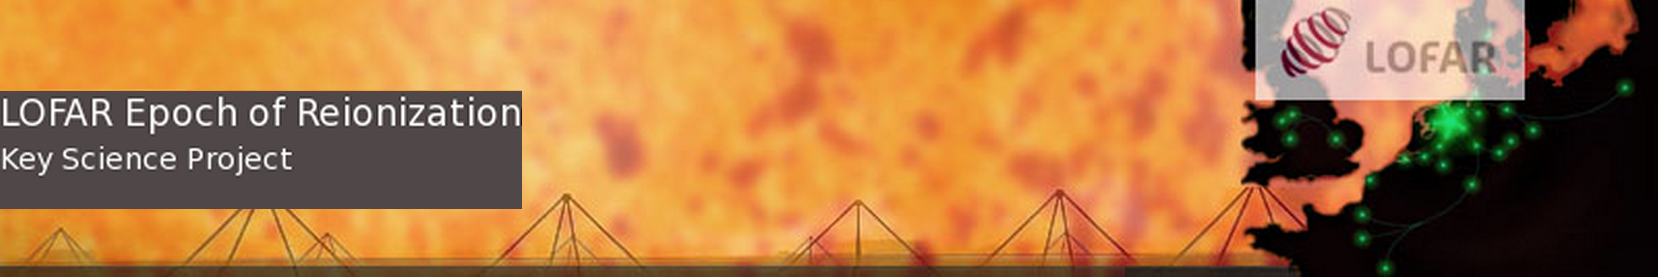
\includegraphics[width=0.8\textwidth]{fig/eorlogo}\\[3cm]    
\textsc{\LARGE Welcome information in the LOFAR EoR processing}\\[0.5cm]
\vfill
{\large 
\emph{Oscar Martinez} \\
University of Groningen \\ 
Kapteyn Astronomical Institute \\
Groningen \\
The Netherlands \\
\today}
\end{center}
\end{titlepage}

\section{Introduction}

First of all, welcome to the LOFAR EoR group, a very international bunch of very smart and particular people. You will have fun. Enjoy!. Now let's talk about business so you can start as soon as possible to help us to find ``the signal". This documents gives a brief introduction in processing the LOFAR EoR data in the LOFAR EoR cluster.

\section{LOFAR EoR cluster}

The LOFAR EoR cluster is the CPU/GPU computer cluster used for the processing of the LOFAR EoR data. 

\subsection*{Account}

The first thing you need is an account in the LOFAR EoR cluster. Contact the system administrator, Eite Tiesinga (tiesinga@astro.rug.nl).

\subsection*{Log in}

Use \textit{ssh} to log in in the portal node (called \textit{lofareor01}) of the LOFAR EoR cluster:

\begin{verbatim}
ssh PRIVATE
\end{verbatim}

From this node you can access any of the nodes of the cluster. 

\subsection*{The nodes}

There are 80 nodes, named \textit{node001} to \textit{node080}, and they are accessed through \textit{ssh}. Each node has 3 disks mounted in \textit{/data1}, \textit{/data2} and \textit{/data3}. Some nodes do not have all the disks and sometimes they break so do not freak out if that happens, it is natural selection. Darwin also applies to data disks.
NFS is also available to access the data in different nodes. For example, if you are in node001 and you want to access the \textit{data1} disk in \textit{node002} you can do it with \textit{/net/node002/data1}. Few comments on the several nodes of the LOFAR EoR cluster:

\begin{itemize}
	\item node001 to node010 can be freely used by the users. New LOFAR EoR users should be using one of them.  However, ask which one you can use. Your life can be in danger if you use the wrong one.
	\item node011 to node074 are reserved for the processing of the project data. Do not use them without consultation. Again, your life can be in the edge.
	\item node075 is used as spare for the main processing nodes and also contains the backup of the LEDDB.
	\item node076 - node080 are nodes recently upgraded that are not functional yet. They should be working soon enough and they are supposed to be super-machines.
\end{itemize}

\subsection*{Using home directory and data disks}

Each user has a home directory in \textit{/home/users/[user name]} that is shared by all the nodes. Do not use it for data storage or processing and never for intensive IO tasks (your life ...). If you want to store large data or do heavy IO tasks, do it in the /data directories of the nodes in a location like \textit{/dataX/users/lofareor/[username]}. You may need to ask the system administration (tiesinga@astro.rug.nl) to create this directory for you in the required nodes.

\section{LOFAR EoR data}

In order to find the EoR signal we require hundreds of observations. A LOFAR EoR observation, which is ten's of terabytes, consists on hundreds of measurement sets. These observations (their measurement sets) need to be processed (flagged, averaged, calibrated, etc.). There are applications for the processing of single measurement sets. There are also tools to ease the processing of a higher number of measurement sets.

\subsection*{Project data}

The project data is stored in node011 to node074, in folders which names are in the format \textit{L[YYYY\_]XXXXX[\_VVV]} where \textit{XXXXX} is the observation identifier, \textit{YYYY} is optional and it is the year of observing and \textit{VVV} indicates the version of the data (if not specified it is 0). These folders are contained in the following directories:

\begin{itemize}
	\item \textit{/dataX/users/lofareor/} for the raw data (version 0)
	\item \textit{/dataX/users/lofareor/pipeline} for the averaged data (version $>$ 0)
\end{itemize}

The data out of these specified locations is not considered project data, we call it user data. Only experienced users should handle/process the project data. Please, ask before trying to use the project data.

The raw project data belongs to the user \textit{lofardata} and only this user and the users in the linux group \textit{lofareor} can modify it.

\section{Data locations: The LEDDB}

We use a database called LEDDB to store the locations of the project data (among other things). 

\subsection*{LEDDB web UI}

When accessing LEDDB web you will be asked for a user name and password, use the same ones that you use to access the LOFAR EoR cluster. Few remarks regarding what the tabs of the LEDDB web UI show:

\begin{itemize}
	\item LDS: the different observations.
	\item LDSB: for each observation, the different beams.
	\item LDSBP: groups, for each beam of each observation, the several measurement sets that are in the same location (LOFAR EoR cluster or any other cluster or archive) and have the same averaging and processing properties.
	\item MS: for each LDSBP entry, the different measurement sets, but only their frequency information.
	\item MSP: for each MS entry, its data location.
	\item GAIN, QTS, QFS and QBS: diagnostic information extracted from the processing of the measurement sets.
	\item GAINMOVIE: locations of Gain solution animations.
\end{itemize}

Selection of rows in a tab will filter the results in other tabs in positions right of the current one. For example, if you select a row in the LDS tab and go to the LDSB tab, you will only see the LDSB rows related to the selected LDS row. In addition, you can filter and sort the rows.

\subsection*{The \textit{RefFile}}

As explained in the previous section, using the LEDDB web UI you can list the observations and the locations of their related data (measurement sets). You can also create a \textit{RefFile}, which is a file that contains the locations of some measurement sets, by selecting some rows in the MSP tab and clicking on \textit{Save RefFile} (you can also create it from other tabs). Be aware that when you create a \textit{RefFile}, it is stored in a temporal location in the LOFAR EoR cluster and you must move it to your home directory (the temporal files are deleted on daily basis so do not complain if the \textit{RefFile} is gone).


\section{Data processing}

The several applications used for the processing of the LOFAR EoR data are:

\begin{itemize}
	\item For flagging: AOFlagger (it can be done in application NDPPP) via the command \textit{rficonsole}.
	\item For averaging: NDPPP (usually we do averaging and flagging in single execution) via the command \textit{NDPPP}.
	\item For calibration: BBS via the command \textit{calibrate-stand-alone}, and SAGECAL via the command \textit{sagecal} (in this case you also need to ``\textit{source /software/users/lofareor/eor-init.sh}'').
	\item For imaging: CASAimager via the command \textit{casapy}, and AWImager via the command \textit{awimager}.
\end{itemize}

\subsection*{Processing many measurement sets}

All the data processing programs presented above are meant to process a single measurement set. You should test them for a while to get a feeling on how they work. Once you have experience in processing a single measurement set there is a tool to help you processing hundreds of them with a single command. Again, only use this tool when you are ``the master" of single measurement set processing.

The tool, which in general requires a \textit{RefFile}, is available by using the LEDDB web UI, through the \textit{Data Manager} button, or by using, in any node of the LOFAR EoR cluster, the command \textit{ExecuteLModule} (use -h to get help). In fact, the web version is just a GUI that helps you filling the parameters required to run the command. Few comments on the tool:

\begin{itemize}
	\item In general this tool will allow you to define some distribution options, i.e. how many simultaneous different nodes are processing measurement sets and how many different measurement sets are simultaneously processed in each node. 
	\item Normally it also allows you to define a logging folder. Each individual execution to a measurement set will log its progress in a file in this folder. If you want to have all the log files in the same folder (which is the usual desire) you should use a location that is shared among all the nodes, for example within your home directory.
	\item In addition there is normally a query mode (usually option -q) that will only show all the commands (that would be executed to all the involved measurement sets) without actually executing them. It is much recommended to use this mode before each execution, specially when you are starting your trip with the LOFAR EoR group.
\end{itemize}

\subsection*{Cluster Monitor}

There is a tool, the \textit{Cluster Monitor}, that shows real-time information of the usage of the nodes. This includes CPU, memory, network traffic and data disks usage. The tool is available in the LEDDB web UI, through the \textit{Cluster Monitor} button. It is also available using the command \textit{ExecuteLModule ClusterMonitor} in any node of the LOFAR EoR cluster. This is particularly handy when you are running something in multiple nodes and want to see what is going on (why there is fire in the nearby building).

\section{Examples}

In the next paragraphs we present a few examples on how to process many measurement sets. We will use a test \textit{RefFile} called \textit{testrefffile.ref}.

Note that we do not specify how many measurement sets are pointed by this \textit{RefFile} so whatever we explain in the following examples is valid for 5 measurement sets but also for 500. 

\subsection{Copying}
Let's assume that the \textit{testrefffile.ref} points to project data. Since we have to be especially careful with the project data, we will first make a copy of the data pointed by the \textit{testrefffile.ref} and do the test processing with the new copies.

When copying the data, in addition to the input \textit{RefFile}, you need to specify the nodes where the data will be copied and the new location in them.

\begin{verbatim}
ExecuteLModule CopyData -i testrefffile.ref -o myrefffile.ref
-u node001-004 -c /data1/users/lofareor/martinez/test -p 1 -n 2
\end{verbatim}

The execution of the previous command copies all the measurement sets pointed by \textit{testrefffile.ref}. The new measurement sets, which locations will be described in \textit{myrefffile.ref}, are distributed in 4 nodes (node001 to node004) and they are copied in the folder 

\textit{/data1/users/lofareor/martinez/test}. Only two nodes are simultaneously receiving new measurement sets and only one at a time.

\subsection{Flagging}

For flagging the data we normally use NDPPP (adding a flag step in the NDPPP parset). However, there is also a command to ``only" run the flagger. In addition to the input \textit{RefFile} you need to specify an execution path where some temporal files are created. Do not use the home directory for this purpose. 

\begin{verbatim}
ExecuteLModule LaunchAOFlagger -i myrefffile.ref 
-e /data1/users/lofareor/martinez/tempflag -l logsflag
\end{verbatim}

The execution of the previous command runs the AOFlagger to all the measurement sets pointed by \textit{myrefffile.ref}. The used nodes are the ones that contain the data. Each of these nodes will use the folder \textit{/data1/users/lofareor/martinez/tempflag} as execution path (it is created if it does not exist). In this case all the processes running in the used nodes will log their progress in \textit{logsflag}.

\subsection{Averaging (and flagging) with NDPPP}

NDPPP requires a parset file that describes where is the measurement set and what processing must be done. Hence, in order to run NDPPP on many measurement sets, first you need to create parset files for all the measurement sets to be processed. There is a command that given a template parset will create a new parset file for each measurement set pointed by a \textit{RefFile} .

\begin{verbatim}
ExecuteLModule CreateNDPPPParsetFiles -i myrefffile.ref 
-t /home/users/martinez/NDPPP/template.parset 
-o /home/users/martinez/NDPPP/parsets -c /data3/users/lofareor/martinez/averagetest
\end{verbatim}

The execution of the previous command will create a parset file for each measurement set pointed by \textit{myrefffile.ref}. The new parset files are stored in \textit{/home/users/martinez/NDPPP/parsets} and they are copies of the template \textit{/home/users/martinez/NDPPP/template.parset}, only that, in each case, it changes the part describing the location of the data. The input measurement set location is given by the input \textit{RefFile} and the output measurement set will be stored in the specified path, i.e. \textit{/data3/users/lofareor/martinez/averagetest}. Once the new parsets are created you can use:
\begin{verbatim}
ExecuteLModule LaunchNDPPP -i /home/users/martinez/NDPPP/parsets -l logsndppp
\end{verbatim}

The execution of the previous command will execute NPPPP for all the parsets that we just created. The output data will be written in the same nodes than the input data (in the path indicated when creating the parsets). If you wish to write the output data in different nodes you can specify it when running the \textit{ExecuteLModule LaunchNDPPP}. In this example all the NDPPP processes will log their progress in \textit{logsndppp}.

After the completion of the previous execution, you will have created new data. You may need a new \textit{RefFile} to do more processing to the data you just created:

\begin{verbatim}
ExecuteLModule CreateRefFileFromPath -i /data3/users/lofareor/martinez/averagetest
 -s node001-004 -o myreffileavg.ref
\end{verbatim}

The execution of the previous command will create a new \textit{RefFile} with all the measurement sets in node001 to node004 contained in the path \textit{/data3/users/lofareor/martinez/averagetest}. The new \textit{RefFile} is called 
\textit{myreffileavg.ref}.

\subsection{Calibrating with BBS}

Running BBS is slightly easier than NDPPP because it does not require to create a parset for each measurement set. It does need a parset file but the same one is used for all the measurement sets. In addition to the input \textit{RefFile}, the parset file and the sky model file, you need to specify an execution path where some temporal files are created. Do not use the home directory for this purpose. 

\begin{verbatim}
ExecuteLModule LaunchCalibrateSA -i myreffileavg.ref 
-e /data1/users/lofareor/martinez/tempbbs 
-a /home/users/martinez/BBS/parset -m /home/users/martinez/BBS/sky -l logsbbs
\end{verbatim}

The execution of the previous command calibrates all the measurement sets pointed by \textit{myreffileavg.ref}. The exact calibration is defined in the parset \textit{/home/users/martinez/BBS/parset}. The used sky model is read from the file \textit{/home/users/martinez/BBS/sky}. In each node with data it will use the folder \textit{/data1/users/lofareor/martinez/tempflag} as execution path, so this path will be created in all the used nodes. In this case all the processes running in the used nodes will log their progress in \textit{logsbbs}.

\subsection{Calibrating with SAGECAL}

SAGECAL needs, in addition to the input \textit{RefFile}, a sky model file (like in BBS) and a cluster file.

\begin{verbatim}
ExecuteLModule LaunchSagecal -i myreffileavg.ref
-s /home/users/martinez/SAGECAL/sky -c /home/users/martinez/SAGECAL/cluster
\end{verbatim}

The execution of the previous command calibrates all the measurement sets pointed by \textit{myreffileavg.ref}. The used sky model is read from the file \textit{/home/users/martinez/SAGECAL/sky} and the cluster information is extracted from the file \textit{/home/users/martinez/SAGECAL/cluster}.

\subsection{Imaging with the CASAImager}

In this example we do imaging with the CASAImager even though it is not the only imager available.
Like NDPPP, the CASAImager requires a parset file that describes where is the measurement set and how the imaging must be done. Hence, in order to run CASAImager on many measurement sets, first you need to create parset files for all the measurement sets. There is a command that given a template parset will create a new parset file for each measurement set pointed by a \textit{RefFile}.

\begin{verbatim}
ExecuteLModule CreateCASAImagerParsetFiles -i myreffileavg.ref 
-o /home/users/martinez/CASA/parsets -t /home/users/martinez/CASA/template.parset
\end{verbatim}

The execution of the previous command will create a parset file for each measurement set pointed by \textit{myreffileavg.ref}. The new parset files are stored in \textit{/home/users/martinez/CASA/parsets} and they are copies of the template \textit{/home/users/martinez/CASA/template.parset}, only that, in each case, it changes the part describing the location of the input data. The input measurement set location is given by the input \textit{RefFile}. The location of the generated images is specified when running the CASAImager. Once the new parsets are created you can use:

\begin{verbatim}
ExecuteLModule LaunchCASAImager -i myreffileavg.ref 
-p /home/users/martinez/CASA/parsets -o /data3/users/lofareor/martinez/images
-l logscasa
\end{verbatim}

The execution of the previous command will execute CASAImager for all the parsets that we just created. The output images will be written in the same nodes than the input data in the path \textit{/data3/users/lofareor/martinez/images}. If you wish to write the output images in different nodes you can specify it when running the \textit{ExecuteLModule LaunchCASAImager}. In this example all the CASAImager processes will log their progress in \textit{logscasa}.

\end{document}
